%\title{Complexe getallen}

\subsection*{Inleiding}
\addcontentsline{toc}{subsection}{Inleiding}

De verzameling van de complexe getallen $\mathbb{C}$ is een uitbreiding van de verzameling van de re\"{e}le getallen $\mathbb{R}$ waarbij elk complex getal bestaat uit twee re\"{e}le getallen. Het ene re\"{e}el getal wordt het re\"{e}el deel van het complex getal genoemd, het andere re\"{e}el getal het imaginaire deel.\\ 
Alhoewel een eerste kennismaking met complexe getallen heel wat mensen hun wenkbrauwen doet fronsen blijkt dit soort getallen heel wat rekenwerk in de fysica en de techniek eenvoudiger te maken. Dit is bijvoorbeeld zeker het geval in vakgebieden als mechanica (trillingen), akoestiek (golven) en elektrotechniek (wisselstroom).\\

\subsection{De imaginaire eenheid}

\begin{definitie}
	Als eerste stap bij het bespreken van complexe getallen defini\"{e}ren we de imaginaire eenheid $i$ als het getal waarvoor geldt:

\[
i^2 =-1 
\]
\end{definitie}

\begin{opmerking}
	Hierbij moeten we enkele bedenkingen maken:\\
\begin{itemize}
\item Het gebeurt wel eens dat deze definitie wordt herschreven als $i=\sqrt{-1}$. Dit is echter totaal {\bf fout}. We zullen verderop zien dat $-1$ meer dan \'{e}\'{e}n vierkantswortel heeft.
\item In sommige vakgebieden zoals elektrotechniek geeft men de voorkeur aan de letter $j$ als symbool voor de imaginaire eenheid.
\item Een eigenschap van $i$ die heel wat rekenwerk kan vereenvoudigen is het volgende:
\begin{eigenschap}
\begin{equation*}
 i^2=-1 \iff  i=-\frac{1}{i} \iff -i=\frac{1}{i} 
\end{equation*}
\end{eigenschap}

\end{itemize}
\end{opmerking}
\subsection{Het complex getal}

\begin{definitie}
Twee re\"{e}le getallen $x$ en $y$ worden gecombineerd tot een complex getal $z$:
\begin{equation*}
z=x+iy
\end{equation*}
\end{definitie}

Het re\"{e}le getal $x$ wordt het re\"{e}le deel van $z$ genoemd: $x=Re(z)=\Re(z)$.\\
Het re\"{e}le getal $y$ wordt het imaginaire deel van $z$ genoemd: $y=Im(z)=\Im(z)$.\\
Merk op dat als $y=0$ dan $z=x$ met $x \in \mathbb{R}$. Met andere woorden de verzameling van de re\"{e}le getallen is een deelverzameling van de verzameling van de complexe getallen: $\mathbb{R} \subset \mathbb{C}$. Analoog geldt dat als $x=0$ dan $z=iy$. Het getal $iy$ wordt een {\bf imaginair getal} genoemd.\\

Aangezien een complex getal bestaat uit twee re\"{e}le getallen kan een complex getal meetkundig worden voorgesteld door een punt in een vlak. Dit vlak, {\bf het complex vlak}, wordt bepaald door de getallenas van de re\"{e}le getallen, de re\"{e}le as, met loodrecht daarop de imaginaire as. Deze laatste is de re\"{e}le as waarop de eenheid (het getal $1$) vervangen is door $i$.  

\gewonefiguur{scale=0.6}{3_gonio_complexe_getallen/inputs/complex-getal-1.jpg}

%\begin{figure}[h]
%\begin{center}
%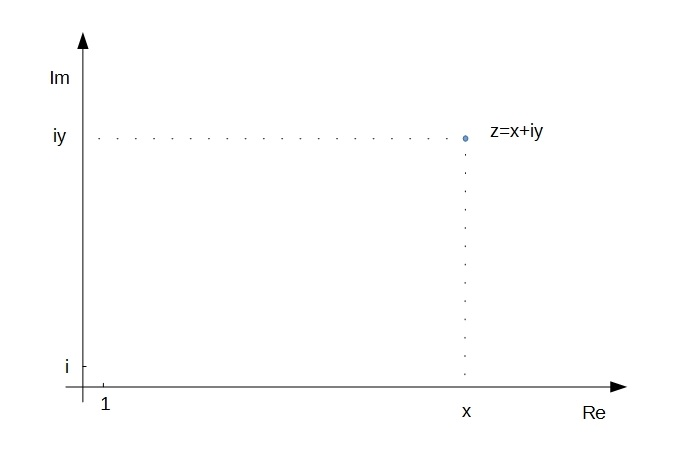
\includegraphics[scale=0.6]{3_gonio_complexe_getallen/inputs/complex-getal-1.jpg}
%\end{center}
%\caption{\it Voorstelling van een complex getal $x+iy$ in het complex vlak}
%\end{figure}

Met behulp van schuifknoppen kan je in de volgende interactieve voorstelling het re\"{e}le en imaginaire deel van het getal veranderen en nagaan waar in het complex vlak het complex getal zich bevindt.\\


\begin{minipage}{.25\linewidth}
	\raggedright
	
\includegraphics[width=4cm]{3_gonio_complexe_getallen/inputs/QR_Code_ANIMATIE1_module3}
\end{minipage}
\begin{minipage}{.7\linewidth}
	Scan QR code voor animatie.
\end{minipage}\\

De plaats van een punt in een vlak is ook bepaald door de plaatsvector van het punt. Een complex getal $z$ kan dus ook worden voorgesteld als een vector in het complex vlak. Een dergelijke vector wordt meestal aangeduid met het symbool $\underline{z}$.\\

\gewonefiguur{scale=0.6}{3_gonio_complexe_getallen/inputs/complex-getal-2.jpg}

Een interactieve voorstelling van een vector in het complex vlak.\\

\begin{minipage}{.25\linewidth}
	\raggedright
	
\includegraphics[width=4cm]{3_gonio_complexe_getallen/inputs/QR_Code_ANIMATIE2_module3}
\end{minipage}
\begin{minipage}{.7\linewidth}
	Scan QR code voor animatie.
\end{minipage}  \\

\subsection{Rekenen met complexe getallen}

\subsubsection{Som van complexe getallen}

\begin{definitie}
De som van twee complexe getallen $z_{1}=a+ib$ en $z_{2}=c+id$ is gedefinieerd als\\

\begin{framed}
\[ z_{1}+z_{2}=(a+c)+i(b+d) \]
\end{framed}

ofwel

\begin{framed}
\[	
\begin{array}{ccc}
\Re(z_{1}+z_{2})=\Re(z_{1})+\Re(z_{2}) &  & \Im(z_{1}+z_{2})=\Im(z_{1})+\Im(z_{2}) 
\end{array} 
\]
\end{framed}
\end{definitie}

Het afzonderlijk optellen van de re\"{e}le en imaginaire delen van de complexe getallen kan beschouwd worden als het optellen van componenten van vectoren in het complex vlak. Met andere woorden: optellen van complexe getallen komt neer op optellen van vectoren in het complex vlak.\\

\gewonefiguur{scale=0.6}{3_gonio_complexe_getallen/inputs/complex-getal-3-optelling.jpg}

%\begin{figure}[h]
%	\begin{center}
%		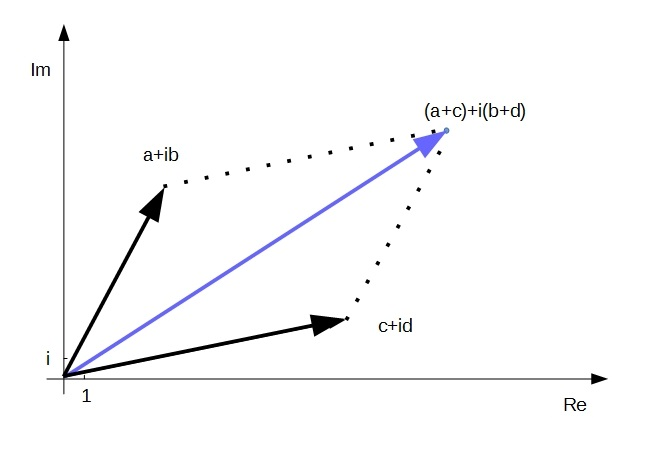
\includegraphics[scale=0.6]{3_gonio_complexe_getallen/inputs/complex-getal-3-optelling.jpg}
%	\end{center}
%\caption{\it Optellen van complexe getallen komt neer op optellen van vectoren in het complex vlak}
%\end{figure}

\subsubsection{Product van complexe getallen}

Als we twee complexe getallen $z_{1}=a+ib$ en $z_{2}=c+id$ met elkaar willen vermenigvuldigen kunnen we dit in eerste instantie neerschrijven als $z_{1} z_{2}=(a+ib)(c+id)$.\\
Om het product te berekenen worden de haakjes uitgewerkt op de klassieke manier maar wordt er expliciet rekening gehouden met $i^2 =-1$.\\

\begin{eigenschap}
	\begin{framed}
\[ z_{1}z_{2}=(a+ib)(c+id)=ac+iad+ibc+i^2 bd=(ac-bd)+i(ad+bc) \]
\end{framed}
\end{eigenschap}

\subsubsection{Complex toegevoegde van een complex getal}

\begin{definitie}
	De complex toegevoegde van een complex getal vindt men door het imaginair deel van een complex getal van teken te veranderen. Men noteert de complex toegevoegde van $z$ als $\overline{z}$.\\
Dus, als $z=x+iy$ dan is de complex toegevoegde van $z$ het getal $\overline{z}=x-iy$.\\
\end{definitie}
\begin{eigenschap}
	Een getal vermenigvuldigen met zijn complex toegevoegde geeft het volgende interessante resultaat:

\begin{framed}
\[ z \overline{z}=(x+iy)(x-iy)=x^2 -ixy+iyx-i^2 y^2=x^2 +y^2 \in \mathbb{R} \]
\end{framed}
\end{eigenschap}

\gewonefiguur{scale=0.6}{3_gonio_complexe_getallen/inputs/complex-getal-4-complex-toegevoegde.jpg}

Een meer interactieve voorstelling vind je hier.\\

\begin{minipage}{.25\linewidth}
	\raggedright
	
\includegraphics[width=4cm]{3_gonio_complexe_getallen/inputs/QR_Code_ANIMATIE3_module3}
\end{minipage}
\begin{minipage}{.7\linewidth}
	Scan QR code voor animatie.
\end{minipage}  \\


\subsubsection{Modulus van een complex getal}

\begin{definitie}
	De grootte van de plaatsvector van een complex getal wordt de modulus van dat getal genoemd. 

\end{definitie}
Met behulp van de stelling van Pythagoras wordt de grootte berekend als $|\underline{z}|=|x+iy|=\sqrt{x^2 +y^2}$.\\
\begin{eigenschap}
	De modulus van het complex getal $z=x+iy$ kan dus ook geschreven worden als

\begin{framed}
\[ |z|=\sqrt{x^2 +y^2}=\sqrt{z \overline{z}}  \]
\end{framed}

\end{eigenschap}

\subsubsection{Quoti\"{e}nt van complexe getallen}

Het berekenen van het quoti\"{e}nt van twee complexe getallen komt er op neer dat men er voor zorgt dat de noemer van de uitdrukking een re\"{e}el getal wordt. De gehele uitdrukking wordt dan een duidelijk leesbaar complex getal.\\
De eenvoudigste manier om dit te doen is teller en noemer vermenigvuldigen met de complex toegevoegde van de noemer.\\
Laten we de getallen $z_{1}=a+ib$ en $z_{2}=c+id$ delen door elkaar:

\begin{framed}
\[ \frac{z_{1}}{z_{2}}=\frac{a+ib}{c+id}=\frac{(a+ib)(c-id)}{(c+id)(c-id)}=\frac{(ac+bd)+i(bc-ad)}{c^2 +d^2}  \]
\end{framed}

\begin{voorbeeld}	
\[ \frac{4-i}{1+i}=\frac{(4-i)(1-i)}{(1+i)(1-i)}=\frac{4-4i-i-1}{2}=\frac{3}{2}-\frac{5}{2}i \]
\end{voorbeeld}

\subsection{Rekenen met complexe getallen - voorbeeld}
\begin{minipage}{.25\linewidth}
	\raggedright
	
\includegraphics[width=4cm]{3_gonio_complexe_getallen/inputs/QR_Code_REKENENCOMPLVB_module3}
\end{minipage}
\begin{minipage}{.7\linewidth}
	Zie filmpje MOOC.
\end{minipage}

\subsection{Goniometrische vorm van een complex getal}

De plaats van een punt $P$ in een vlak wordt traditioneel vastgelegd met behulp van de cartesische co\"{o}rdinaten $(x,y)$. Het is echter evengoed mogelijk hiervoor andere co\"{o}rdinaten te kiezen. Een mogelijk alternatieve keuze zijn de afstand $r$ van het punt $P$ tot de oorsprong en de hoek $\theta$ die de rechte $OP$ maakt met de $x-$as. $(r,\theta)$ worden poolco\"{o}rdinaten genoemd.\\
Passen we dit toe op een complex getal $z$ in het complex vlak dat wordt de afstand $r$ de modulus $|z|$ en de hoek $\theta$ de hoek die de vector $\underline{z}$ maakt met de $x-$as.\\

\begin{figure}[h]
	\begin{center}
		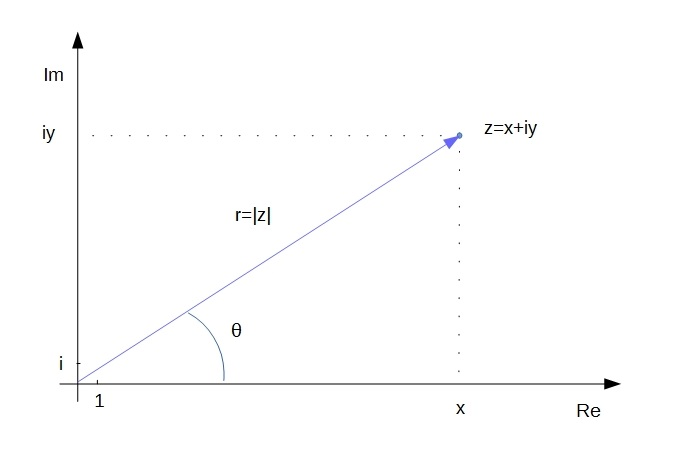
\includegraphics[scale=0.6]{3_gonio_complexe_getallen/inputs/complex-getal-5-goniometrisch.jpg}
	\end{center}
	\caption{\it Goniometrische vorm van een complex getal. De plaats van het getal in het complex vlak wordt vastgelegd door de poolco\"{o}rdinaten $r=|z|$ en $\theta$}
\end{figure}

Door de bij het getal $z=x+iy$ horende vector te projecteren op de re\"{e}le as en op de imaginaire as vindt men

\[ \left\{ \begin{array}{l}
x=\Re(z)=|z|\cos \theta  \\ y=\Im(z)=|z|\sin \theta
\end{array} \right. \]

\begin{eigenschap}
	In goniometrische vorm wordt dat

\begin{framed}
\[ z=x+iy=|z|(\cos \theta + i \sin \theta)   \]
\end{framed}
Met 

\begin{framed}
	\[ \begin{array}{lll}
	\text{modulus van } z=x+iy & & |z|=\sqrt{x^2 +y^2} \\
	\text{argument van } z=x+iy & & \theta = \arctan \frac{y}{x}
	\end{array} \]
\end{framed}

\end{eigenschap}


\begin{opmerking}
\ \\
\begin{itemize}
	\item Een punt in het complex vlak met $r=|z|$ en poolhoek $\theta$ kan ook beschreven worden met dezelfde $r$ maar een poolhoek $\theta+2\pi$, een poolhoek $\theta+ 4\pi$, enz... Men zegt dat de hoek $\theta$ bepaald is op een geheel aantal keer $2\pi$ na.
	\[ z=|z|(\cos \theta + i \sin \theta)=|z|(\cos(\theta +k2\pi)+i \sin(\theta+k2\pi)) \]
	met $k$ een geheel getal.\\
	De hoek waarvoor geldt $\theta \in [0,2\pi[$ is de {\bf hoofdwaarde van het argument}. 
	\item Bij het berekenen van het argument wordt gebruik gemaakt van de Arctan-functie. Het bereik van deze functie is $]-\frac{\pi}{2},\frac{\pi}{2}[$ waardoor het berekende argument het complex getal altijd in het eerste of vierde kwadrant plaatst.\\ 
	{\bf Het is dus zeer belangrijk om te controleren of het complex getal in werkelijkheid niet in het tweede of derde kwadrant ligt. Als dat het geval is moet een correctie op het berekende argument worden toegepast!} \\ We illustreren hoe dit in zijn werk gaat met enkele voorbeelden.
\end{itemize}

\end{opmerking}

	We zetten de volgende complexe getalen in goniometrische vorm: \\
\begin{voorbeeld}


	$z=3+2i$ \\  We maken een figuur om duidelijk te maken in welk kwadrant het getal ligt. \\
	
	\gewonefiguur{scale=0.5}{3_gonio_complexe_getallen/inputs/complex-getal-voorbeeld1.jpg}
	

	Het getal ligt in het eerste kwadrant. We kunnen dus gewoon de formule voor het argument gebruiken zonder correctie.\\
	\[ \begin{array}{lll}
	|z|=\sqrt{3^2 +2^2} & & |z|=\sqrt{13} \\
	\tan \theta = \frac{2}{3} & & \theta = 33,69^{o}\\
	         & &      \\
	z=\sqrt{13} (\cos (33,69^{o}) + i \sin (33,69^{o})  &  &
	\end{array} \]
\end{voorbeeld}
	
\begin{voorbeeld}
	$z=-3-2i$ \\ We maken een figuur om duidelijk te maken in welk kwadrant het getal ligt. \\
	
	\gewonefiguur{scale=0.5}{3_gonio_complexe_getallen/inputs/complex-getal-voorbeeld2.jpg}
	
	Het getal ligt in het derde kwadrant. We moeten dus een correctie toepassen op het berekende argument $\theta$ om het werkelijke argument $\theta^{'}$ te vinden. We tellen  $\pi$ of $180^{o}$ bij het berekende argument. \\
	\[ \begin{array}{lll}
	|z|=\sqrt{(-3)^2 +(-2)^2} & & |z|=\sqrt{13} \\
	\tan \theta = \frac{-2}{-3}=\frac{2}{3} & & \theta = 33,69^{o}\\
	\theta^{'}=\theta+180^{o} & & \theta^{'}=213,69^{o} \\
	&  &          \\
    z=\sqrt{13} (\cos (213,69^{o}) + i \sin (213,69^{o})) &  & 
	\end{array} \]
\end{voorbeeld}
	
\begin{voorbeeld}
	 $z=-3+2i$ \\ We maken een figuur om duidelijk te maken in welk kwadrant het getal ligt. \\

	\gewonefiguur{scale=0.5}{3_gonio_complexe_getallen/inputs/complex-getal-voorbeeld3.jpg}
	
	Het getal ligt in het tweede kwadrant. We moeten dus een correctie toepassen op het berekende argument $\theta$ om het werkelijke argument $\theta^{'}$ te vinden. We tellen  $\pi$ of $180^{o}$ bij het berekende argument. \\
	\[ \begin{array}{lll}
	|z|=\sqrt{(-3)^2 +2^2} & & |z|=\sqrt{13} \\
	\tan \theta = \frac{2}{-3}=-\frac{2}{3} & & \theta = -33,69^{o}\\
	\theta^{'}=\theta+180^{o} & & \theta^{'}=146,31^{o} \\
	&  &          \\
	z=\sqrt{13} (\cos (146,31^{o}) + i \sin (146,31^{o})) &  & 
	\end{array} \]

\end{voorbeeld}

\subsection{De exponenti\"{e}le vorm van een complex getal}

\subsubsection{De formule van Euler}

De formule van Euler drukt uit hoe de functies $\cos$ en $\sin$ in verband staan met de natuurlijke exponenti\"{e}le functie.\\
\begin{eigenschap}
	Voor elk getal $x \in \mathbb{R}$ geldt:\\

\begin{framed}
	\[ e^{ix}=\cos(x) + i \sin(x) \]
\end{framed}
\end{eigenschap}

Deze formule wordt bewezen in de analyse door aan te tonen dat de Taylorreeksontwikkeling van de functie $e^{ix}$ en van de functie $\cos(x) + i \sin(x)$ hetzelfde zijn. \\

\begin{eigenschap}
	Voor praktisch rekenwerk met complexe getallen wordt de formule van Euler neergeschreven als:\\

\begin{framed}
	\[  \begin{array}{l} 
	e^{i \theta}=\cos \theta +i \sin \theta \\
	e^{-i \theta}=\cos \theta - i \sin \theta 
	\end{array}  \]
\end{framed}
Waarbij $\theta$ het argument voorstelt van de goniometrische vorm van een complex getal. \\
\end{eigenschap}

\begin{eigenschap}
	De formule van Euler leidt dus tot een derde, voor de praktijk zeer belangrijke, schrijfwijze voor complexe getallen.\\

\begin{framed}
	\[ \begin{array}{ll}
	\text{de algebra\"{i}sche vorm} & z=x+iy \\
	\text{de goniometrische vorm} & z=|z|(\cos \theta +i \sin \theta) \\
	\textbf{de exponenti\"{e}le vorm} & z=|z|e^{i \theta} \end{array}  \]
\end{framed}

\end{eigenschap}

In principe moet in de formule van Euler, en dus ook in de exponenti\"{e}le vorm van een complex getal, het argument $\theta$ uitgedrukt worden in radialen. Het gebeurt echter dikwijls dat het argument wordt uitgedrukt in graden. Dit is geen probleem zolang men beseft dat om de {\bf numerieke waarde} van bijvoorbeeld $e^{i 45^{o}}$ rechtstreeks te berekenen men $e^{i\frac{\pi}{4}}$ moet uitrekenen.\\
	

\begin{voorbeeld}
	We schrijven het getal $z=-2\sqrt{3}-2i$ in exponenti\"{e}le vorm.\\

\vspace{0.3cm}

Als eerste stap maken we een figuur die het getal voorstelt in het complex vlak.\\

\gewonefiguur{scale=0.5}{3_gonio_complexe_getallen/inputs/complex-getal-voorbeeld4.jpg}

Het getal ligt in het derde kwadrant. Er zal dus een correctie op de berekende waarde voor het argument moeten worden toegepast.\\

\[ \begin{array}{lll}
	|z|=\sqrt{(-2\sqrt{3})^2 +(-2)^2} & & |z|=4 \\
	\tan \theta = \frac{-2}{-2\sqrt{3}}=\frac{1}{\sqrt{3}} & & \theta = 30^{o}\\
	\theta^{'}=\theta+180^{o} & & \theta^{'}=210^{o} \\
	&  &          \\
	z=4e^{i210^{o}} \text{ of ook } z=4e^{i\frac{7}{6}\pi}  &  & 
\end{array} \]

\end{voorbeeld}

\subsection{Bewerkingen in exponenti\"{e}le vorm: som, product en quoti\"{e}nt} 

\subsubsection{De som}

Er bestaat geen snelle manier om twee complexe getallen in exponenti\"{e}le vorm op te tellen. Als je met dit probleem geconfronteerd wordt kan je op twee manieren te werk gaan.\\

{\bf Eerste werkwijze:} \\

\begin{enumerate}
	\item Reken de complexe getallen om naar hun algebra\"{i}sche vorm met behulp van de formule van Euler
	\item Tel de getallen in algebra\"{i}sche vorm op
	\item Zet de som terug om naar exponenti\"{e}le vorm.
\end{enumerate}

\vspace{0.3cm}

{\bf Tweede werkwijze:} \\

Beschouw het optellen van de twee complexe getallen als het optellen van twee vectoren in het complex vlak en gebruik driehoeksmeetkunde om de grootte (modulus) en de ori\"{e}ntatie (argument) van de somvector te bepalen.\\

\vspace{0.3cm}

Beschouw twee complexe getallen $a=|a|e^{i\alpha}$ en $b=|b|e^{i\beta}$ waarvan je de som wil berekenen. Je wil dus modulus en argument van het complex getal $z=a+b=|z|e^{i\theta}$ vinden.\\
Maak nu een figuur waarin je de optelling grafisch voorstelt als de optelling van vectoren in het complex vlak:\\

\figuurmetlabel[\label{fig:compl_som}]{scale=0.6}{3_gonio_complexe_getallen/inputs/complex-getal-6-optelling-exp.jpg}{Grafische voorstelling van de optelling van twee complexe getallen als optelling van vectoren in het complex vlak. De modulus van de som $z=a+b$ wordt berekend met behulp van de cosinusregel.}

%\begin{figure}[h]
%	\begin{center}
%		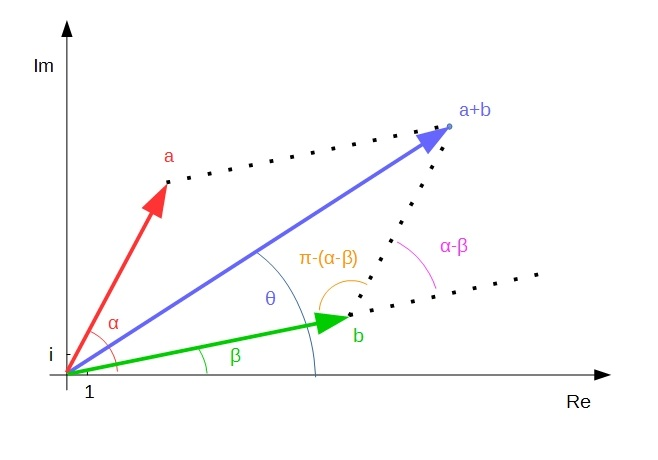
\includegraphics[scale=0.6]{3_gonio_complexe_getallen/inputs/complex-getal-6-optelling-exp.jpg}
%	\end{center}
%	\caption{\it Grafische voorstelling van de optelling van twee complexe getallen als optelling van vectoren in het complex vlak. De modulus van de som $z=a+b$ wordt berekend met behulp van de cosinusregel.}
%\end{figure}

In de driehoek gevormd door de vectoren $\underline{a}$, $\underline{b}$ en de somvector $\underline{z}=\underline{a+b}$ kan je de cosinusregel toepassen om de grootte van $\underline{z}$ te berekenen:\\

\[ |z|^2 =|a|^2 +|b|^2 -2|a||b|\cos(\pi-(\alpha-\beta))  \]

Aangezien $\cos(\pi-(\alpha-\beta))=-\cos(\alpha-\beta)$ kan de modulus van de som $z=a+b$ geschreven worden als:\\

\begin{eigenschap}
	\begin{framed}
	\[ |z|=\sqrt{|a|^2 +|b|^2 +2|a||b|\cos(\alpha-\beta)} \]
\end{framed}
\end{eigenschap}

Het argument $\theta$ van de som  kan je vinden door op de driehoek de sinusregel toe te passen om de hoek tussen de vectoren $\underline{b}$ en $\underline{a+b}$ te berekenen en deze hoek op te tellen bij $\beta$.\\

\vspace{0.2cm}

Je kan ook een algemene maar vrij ingewikkelde formule opstellen voor het argument door met de formule van Euler het re\"{e}ele deel en imaginaire deel van de getallen apart op te tellen.\\

\[  \begin{array}{l}  
\Re(z)=\Re(a)+\Re(b)=|a|\cos \alpha + |b|\cos \beta \\
\Im(z)=\Im(a)+\Im(b)=|a|\sin \alpha + |b|\sin \beta  \end{array} \] 

Het argument vind je via de algemene formule:\\

\begin{eigenschap}
	\begin{framed}
	\[ \tan \theta =\frac{\Im(z)}{\Re(z)}=\frac{|a|\sin \alpha + |b|\sin \beta}{|a|\cos \alpha + |b|\cos \beta}   \]
\end{framed}
\end{eigenschap}

\subsubsection{Het product}

In tegenstelling tot het optellen van complexe getallen in exponenti\"{e}le vorm is het vermenigvuldigen zeer eenvoudig. Men kan gewoon de rekenregels voor het vermenigvuldigen van exponenti\"{e}le functies toepassen.\\

\vspace{0.2cm}

\begin{eigenschap}
	Neem twee getallen $a=|a|e^{i\alpha}$ en $b=|b|e^{i \beta}$. Het product geeft dan:\\

\[  z=|z|e^{i \theta}=ab=(|a|e^{i\alpha})(|b|e^{i \beta})  \]

Dus:\\

\begin{framed}
	\[ z=|z|e^{i \theta}=|a||b|e^{i (\alpha + \beta)}       \]
\end{framed}
\end{eigenschap}

Met andere woorden: de nieuwe modulus wordt gevonden door de twee oorspronkelijke moduli te vermenigvuldigen, en het nieuwe argument wordt gevonden door de oorspronkelijke argumenten op te tellen.\\

\vspace{0.2cm}

Het vermenigvuldigen van twee complexe getallen kan ook grafisch ge\"{i}nterpreteerd worden. De vermenigvuldiging van $a=|a|e^{i\alpha}$ met $b=|b|e^{i\beta}$ komt neer op het veranderen van de lengte van de met $a$ geassocieerde vector gevolgd door het roteren van de nieuwe vector over een rotatiehoek $\beta$.\\

\gewonefiguur{scale=0.6}{3_gonio_complexe_getallen/inputs/product-grafisch.jpg}

%\begin{figure}[ht]
%	\begin{center}
%		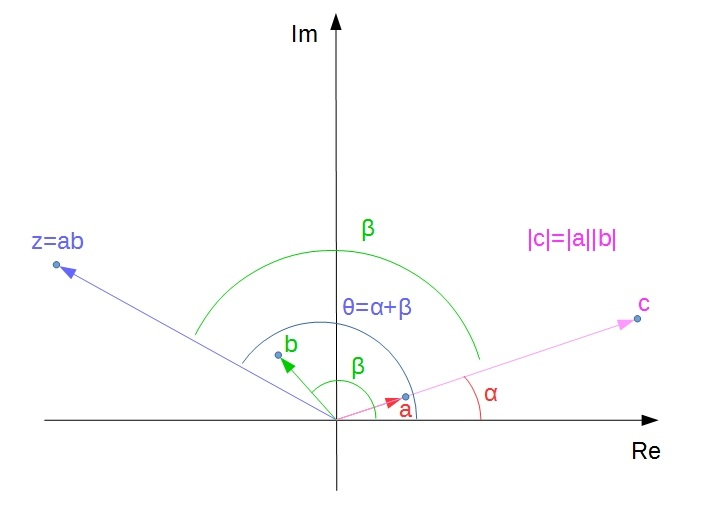
\includegraphics[scale=0.6]{3_gonio_complexe_getallen/inputs/product-grafisch.jpg}
%	\end{center}
%	\caption{\it Grafische interpretatie van het product van $a=|a|e^{i\alpha}$ met $b=|b|e^{i\beta}$.}
%\end{figure}

\begin{itemize}
	\item De met $a=|a|e^{i\alpha}$ en $b=|b|e^{i\beta}$ geassocieerde vectoren in het complex vlak worden voorgesteld in de figuur.
	\item Als eerste stap wordt een nieuw getal $c$ geconstrueerd met hetzelfde argument als $a$ maar met modulus $|c|=|a||b|$. De met $c$ geassocieerde vector ligt dus evenwijdig met de met $a$ geassocieerde vector maar heeft een andere lengte.
	\item Vervolgens wordt de nieuwe vector $\underline{c}$ geroteerd over een hoek $\beta$ wat de vector $\underline{z}$ oplevert. Het met deze vector geassocieerde complex getal $z=|a||b|e^{i(\alpha + \beta)}$ is het product van $a$ en $b$.
\end{itemize}

Deze stappen worden ge\"{i}llustreerd in deze demo:\\

\begin{minipage}{.25\linewidth}
	\raggedright
	
\includegraphics[width=4cm]{3_gonio_complexe_getallen/inputs/QR_Code_ANIMATIE4_module3}
\end{minipage}
\begin{minipage}{.7\linewidth}
	Scan QR code voor animatie.
\end{minipage}    \\

\subsubsection{Het quoti\"{e}nt}

Het complex getal $a=|a|e^{i\alpha}$ delen door het complex getal $b=|b|e^{i\beta}$ gebeurt op analoge manier als bij de vermenigvuldiging:\\

\begin{eigenschap}
	\begin{framed}
	\[ z=\frac{|a|e^{i\alpha}}{|b|e^{i\beta}}=\frac{|a|}{|b|}e^{i (\alpha - \beta)}  \]
\end{framed}
\end{eigenschap}

Grafisch wordt dit ge\"{i}nterpreteerd als het opeenvolgens construeren van een vector $\underline{c}$, evenwijdig met de met $a$ geassocieerde vector en met grootte $|c|=\frac{|a|}{|b|}$, gevolgd door rotatie van de nieuwe vector $\underline{c}$ over een hoek $-\beta$.\\

\subsection{Bewerkingen in exponenti\"{e}le vorm: machtsverheffing en worteltrekking}

\subsubsection{Machtsverheffing}

Een complex getal verheffen tot de macht $n \in \mathbb{N}$ kan je beschouwen als een speciaal geval van het vermenigvuldigen van complexe getallen. Het getal $z$ wordt $n$ keer met zichzelf vermenigvuldigd. Dus:\\

\begin{definitie}
	\begin{framed}
\begin{equation*}
\text{Voor } z \in \mathbb{C} \text{ met } z = |z|e^{i\theta} \text{ en } n \in \mathbb{Z} \text{ geldt } \\
z^n = (|z|e^{i \theta})^n = |z|^n e^{i n \theta}.
\end{equation*}
\end{framed}
\end{definitie}
%
%
%Dus:\\
%
%\begin{framed}
%	\[ z^n =|z|^n e^{i n \theta} \]
%\end{framed}

\begin{opmerking}
	

\begin{itemize}
	\item Door de uitdrukking $(e^{i \theta})^n = e^{i n \theta}$ om te zetten naar goniometrische vorm met de formule van Euler vindt men
	\begin{eigenschap}
		\[  (\cos \theta + i \sin \theta)^n = \cos (n\theta)+i \sin(n \theta) \]
	\end{eigenschap}
	Deze uitdrukking staat bekend als de {\bf formule van de Moivre }. 
	\item Zelfs als een complex getal gegeven is in algebra\"{i}sche vorm is het voor de machtsverheffing meestal aan te raden om het getal om te zetten in exponenti\"{e}le vorm.\\
	\[ (1+i)^5 = (1+i)(1+i)(1+i)(1+i)(1+i)=... \]
	In exponenti\"{e}le vorm (het getal ligt in het eerste kwadrant):\\
	\[ (1+i) = \sqrt{(1^2 + 1^2)} e^{i \arctan{1}}    \]
	dus
	\[  (1+i)= \sqrt{2} e^{i \frac{\pi}{4}} \]
	Machtsverheffing:
	\[ \begin{array}{l} (1+i)^5 = (\sqrt{2})^5 e^{i \frac{5}{4} \pi}= 4\sqrt{2}e^{i \frac{5}{4} \pi} \\
	(1+i)^5 = 4\sqrt{2} (\cos(\frac{5}{4} \pi)+i\sin(\frac{5}{4} \pi)) \\
	(1+i)^5 = 4 (-1 -i) \\
	(1+i)^5 = -4-4i \end{array}  \]
	
\end{itemize}

\end{opmerking}
\subsubsection{Worteltrekking}

\begin{definitie}
	Een $n-$de machtswortel $z_n$ van een complex getal (met $n \in \mathbb{N}$ ) wordt als volgt gedefinieerd:\\

\begin{framed}
	\[  z_{n} \text{ is {\bf een} } n-\text{de machtswortel van } z \in \mathbb{C} \iff (z_{n})^n = z  \] 
\end{framed}
\end{definitie}

Om de wortels te vinden schrijven we de complexe getallen in exponenti\"{e}le notatie en drukken we expliciet uit dat het argument op een geheel aantal keer $2 \pi$ na bepaald is.\\

\[ \begin{array}{ll} 
\text{het complex getal in exponenti\"{e}le vorm} & z=|z|e^{i(\theta +k 2 \pi)}, k \in \mathbb{Z} \\
\text{een n-de machtswortel van } z & z_{n}=|z_{n}|e^{i \theta_{n}}
\end{array}
\]

Toepassen van de definitie geeft:\\

\[ \begin{array}{l}
(|z_{n}|e^{i \theta_{n}})^n = |z|e^{i(\theta + k 2 \pi)} \\
\iff |z_{n}|^n e^{i n \theta_{n}} = |z|e^{i(\theta + k 2 \pi)} \\ 
\iff |z_{n}|=\sqrt[n]{|z|} \text{ en } \theta_{n,k}=\frac{\theta + k 2 \pi}{n}, k=0,1,2,...,n-1 
\end{array} 
\]

Er zijn maar $n$ verschillende waarden voor $k$ want zodra $k=n$ bekomt men hetzelfde argument als voor $k=0$:

\[ \begin{array}{l}   
k=0 \iff \theta_{n,0}=\frac{\theta}{n} \\
\\
k=n \iff \theta_{n,n}=\frac{\theta + n 2\pi}{n}=\frac{\theta}{n} + 2\pi
\end{array}
\]

\begin{ftonthoud}
	
	Elk complex getal $z=|z|e^{i \theta}$ heeft $n$ verschillende $n-$de machtswortels:\\
	\[ z_{n,k}=\sqrt[n]{|z|}e^{i\frac{\theta+k2 \pi}{n}}  \] 
	met $k=0,1,...,n-1$

\end{ftonthoud}


\begin{voorbeeld}
	Bereken de tweedemachtswortels van $z=-1$ (m.a.w. $\sqrt{-1}$).\\
	
	\vspace{0.5cm}
	
	We schrijven $-1$ eerst in exponenti\"{e}le vorm:
	\[ z=-1 \iff z=1 e^{i\pi} \iff z=e^{i(\pi+k2\pi)}, k\in\mathbb{Z} \]
	We passen de definitie van $2-$de machtswortel toe:
	\[ \begin{array}{l} 
	(|z_{2}| e^{i \theta_{2}})^2 = e^{i(\pi + k2\pi)}  \\
	\iff |z_{2}|^2 e^{i2\theta_{2}} = 1e^{i(\pi + k2\pi)} \\
	\iff   \left\{ \begin{array}{l} |z_{2}|^2 =1 \\
	2\theta_{2}=\pi +k2\pi, k\in \mathbb{Z} \end{array} \right.
	\iff \left\{ \begin{array}{l} |z_{2}|=1 \\
	\theta_{2}=\frac{\pi + k2\pi}{2}, k=0,1 \end{array} \right.
	\end{array} 	  \]
	De twee tweedemachtswortels van $z=-1$ zijn dus
	\[  \left\{ \begin{array}{l} z_{2,0}=1e^{i\frac{\pi}{2}}= i \\
	z_{2,1}=1e^{i\frac{3\pi}{2}} = -i
	\end{array} \right.				 	
	\]
	
	Het complex getal $z=-1$ heeft dus {\bf twee} vierkantswortels: $i$ en $-i$. De in technische teksten veel gebruikte uitdrukking $i=\sqrt{-1}$ is dus {\bf niet correct}... 
\end{voorbeeld}
\begin{voorbeeld}
	Bereken de derdemachtswortels van 125: $\sqrt[3]{125}=?$ .\\
	
	\vspace{0.5cm}
	
	We beschouwen $z=125$ als een complex getal en schrijven het in exponenti\"{e}le vorm: $z=125e^{i(0+k2\pi)}, k\in\mathbb{Z}$\\ Dan gebruiken we de definitie van de derde machtswortels: $(z_{3})^3 =125$ \\
	
	\[ \begin{array}{l} 
	|z_{3}|^3 e^{i3\theta_{3}} = 125e^{ik2\pi} 
	\iff |z_{3}|=\sqrt[3]{125}=5 \text{ and } \theta_{3}=k\frac{2\pi}{3}, k=0,1,2 
	\end{array} 
	\]
	
	De derdemachtswortels van $125$ zijn dus:\\
	
	\[  \left\{  \begin{array}{l}
	z_{3,0}=5 \\ z_{3,1}=5e^{i\frac{2\pi}{3}} \\ z_{3,2}=5e^{i\frac{4\pi}{3}} \end{array} \right.	
	\]
	
	\gewonefiguur{scale=0.6}{3_gonio_complexe_getallen/inputs/derdemachtswortels-voorbeeld.jpg}
	
	In het complex vlak liggen de wortels op een cirkel met de oorsprong als middelpunt en met straal $|z_{3}|$. De argumenten van de verschillende wortels zijn zodanig dat de drie wortels op de hoekpunten van een gelijkzijdige driehoek liggen.\\
	
\end{voorbeeld}

Dit laatste kan veralgemeend worden. De n verschillende n-de machtswortels van een complex getal liggen allemaal op een cirkel met middelpunt de oorsprong van het complex vlak. De wortels vormen de hoekpunten van een gelijkzijdige n-hoek.\\

%\end{itemize}

\subsection{Toepassing: fasoren}

Een complex getal $z=|z|e^{i\theta}$ komt meetkundig overeen met een punt in het complex vlak. De plaats van dat punt wordt aangeduid met een vector in het complex vlak.\\
Door nu het argument van het complex getal te veranderen als functie van de tijd, bijvoorbeeld $\theta= \omega t + \alpha$, kan met de vector laten roteren met hoeksnelheid $\omega$ in het complex vlak, $\alpha$ komt dan overeen met het argument op tijdstip $t=0$.\\
Een roterende vector in het complex vlak noemt men een {\bf fasor}.\\

Hier is een fasor met beginfase $\alpha=\frac{\pi}{4}$ voorgesteld:\\

\begin{minipage}{.25\linewidth}
	\raggedright
	
\includegraphics[width=4cm]{3_gonio_complexe_getallen/inputs/QR_Code_ANIMATIE5_module3}
\end{minipage}
\begin{minipage}{.7\linewidth}
	Scan QR code voor animatie.
\end{minipage}    \\   \\

Fasoren kennen veel toepassingen, zo worden ze gebruikt in de elektrotechniek bij rekenwerk met wisselspanning, en in de mechanica bij de beschrijving van trillingen. \\ 
Met de formule van Euler kan bijvoorbeeld een wisselspanning $V=V_{0}\cos(\omega t + \alpha)$ even goed geschreven worden als $V=\Re (V_{0}e^{i(\omega t + \alpha)}) $. Bovendien is rekenen met de exponenti\"{e}le functie $e^{i\theta}$ dikwijls eenvoudiger dan rekenen met de $\cos$ of $\sin$ functies. Daarom wordt in elektrotechniek dikwijls gebruik gemaakt van de complexe spanning $V=V_{0}e^{i(\omega t + \alpha)}$, de werkelijke, fysische spanning vindt men dan door het re\"{e}le deel van de complexe spanning te nemen.\\
Een complexe wisselspanning of wisselstroom kan dus voorgesteld worden door een fasor waarvan het re\"{e}le deel, dus de projectie op de re\"{e}le as, de fysische spanning voorstelt.  Op dezelfde manier kan men in de mechanica van trillingen werken met complexe plaatsco\"{o}rdinaten en complexe snelheden.\\

Hier zie je een fasor met de projecties op de re\"{e}le en imaginaire as en de voorstelling van het re\"{e}le en imaginaire deel als functie van de tijd. \\

\begin{minipage}{.25\linewidth}
	\raggedright
	
\includegraphics[width=4cm]{3_gonio_complexe_getallen/inputs/QR_Code_ANIMATIE6_module3}
\end{minipage}
\begin{minipage}{.7\linewidth}
	Scan QR code voor animatie.
\end{minipage}    \\     \\

Een gedempte trilling met startamplitude $u_{0}$ wordt beschreven door een fasor $u(t)=u_{0}e^{-\alpha t}e^{i\omega t}$. Het re\"{e}le deel van $u(t)$ beschrijft dan de fysische trilling. Hierbij kan $u(t)$, afhankelijk van de toepassing, zowel een spanning, een plaatsco\"{o}rdinaat, een snelheid of nog een andere grootheid voorstellen.\\

\begin{minipage}{.25\linewidth}
	\raggedright
	
\includegraphics[width=4cm]{3_gonio_complexe_getallen/inputs/QR_Code_ANIMATIE7_module3}
\end{minipage}
\begin{minipage}{.7\linewidth}
	Scan QR code voor animatie.
\end{minipage}   \\

\subsection{Test complexe getallen}
TODO